\section{Pushing
\passage{Insomnia}}

    \begin{marginfigure}
\checkoddpage \ifoddpage \forcerectofloat \else \forceversofloat \fi
\centering
 \frame{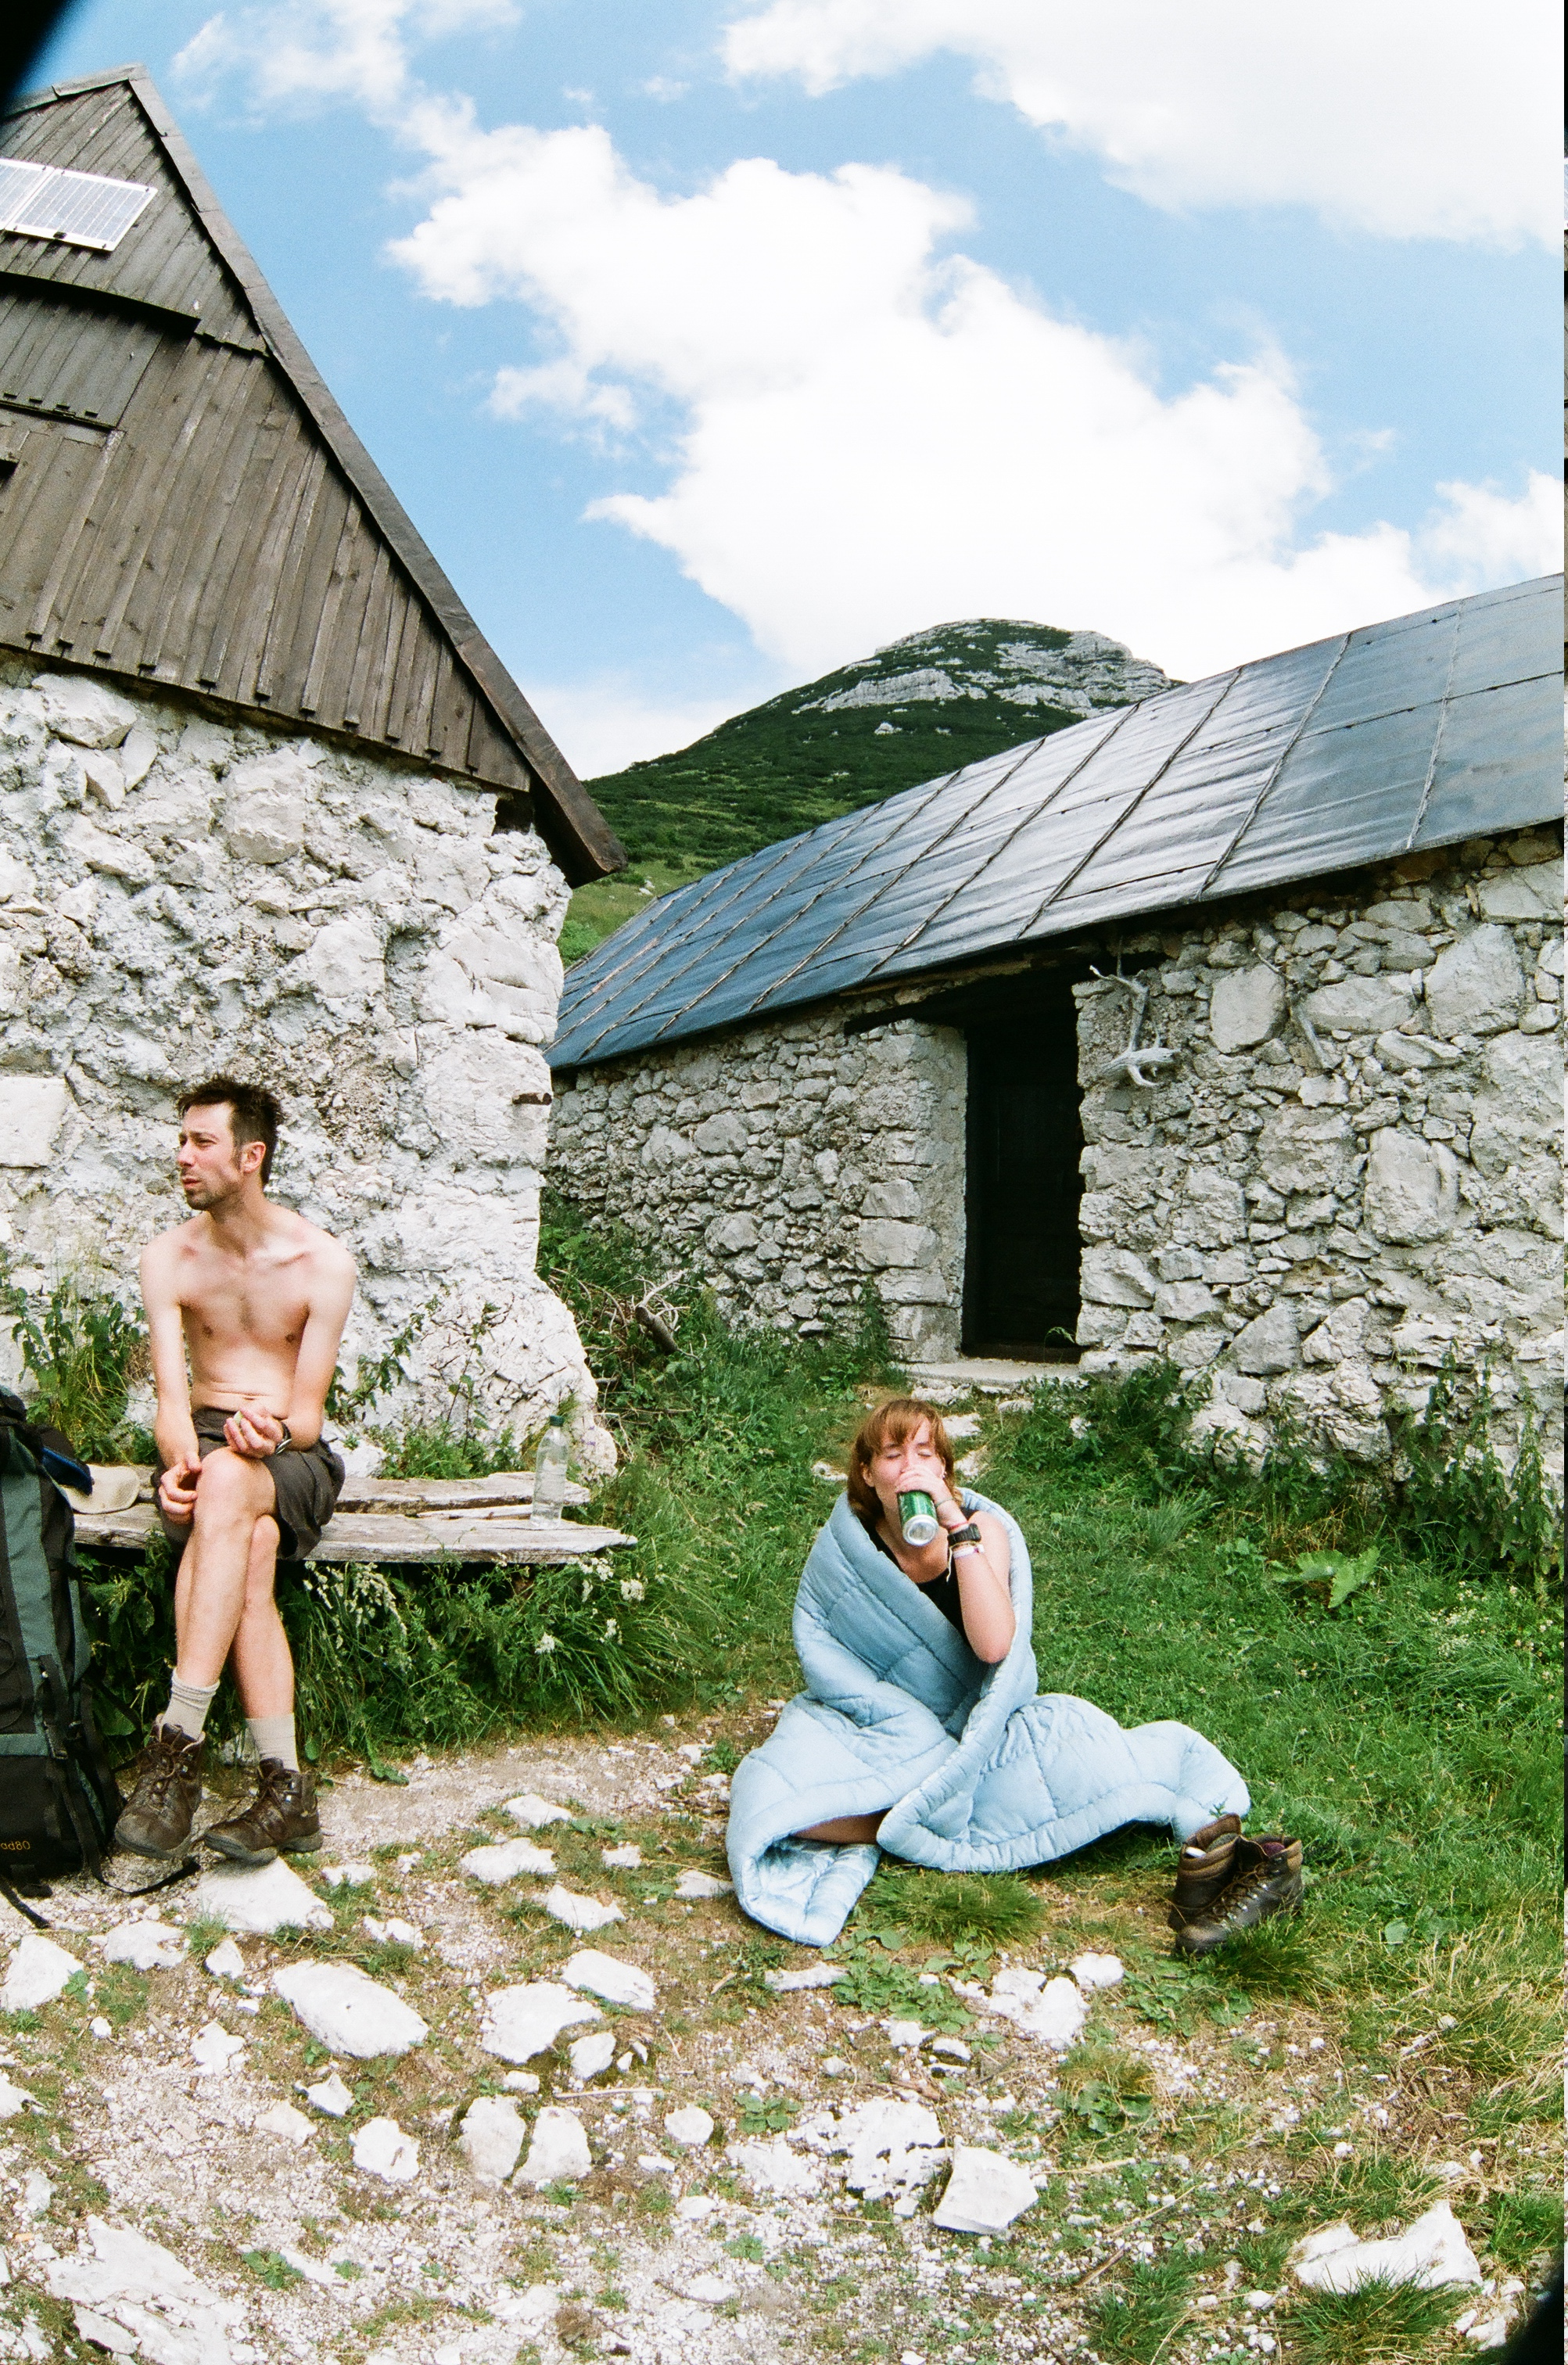
\includegraphics[width=\linewidth]{2010/insomnia/Jarvist Frost - Canon A1 Zenit 16mm - 61320015--orig.jpg}} 
 \caption{James Kirkpatrick and Kate Smith enjoying a break at \passage{Planina Kal}. \pic{Jarvist Frost}}
 \label{quilt kal}
\end{marginfigure}

I had travelled down to \passage[town]{Tolmin} to clean and get over the cabin fever that
develops over the weeks of life on the \passage{Plateau}. That night, after a slap
up meal and a few bruskies, Jan arrived and we had a great evening of
beer and bullshit. After the beer, we passed on to the whiskey and the
bullshit got increasingly epic. ''The leads at the bottom of \passage{Red
Cow} are going to make GW deeper,'' I told Jan. ''The next pushing trip
will definitely do it.'' So after walking up the hill having dinner and
a little too much to drink at the \passage{bivi} we set off for the night train.

Soon enough we are at camp and decide to keep going down, looking to
continue pushing the \passage{Republika} lead. I must admit it took a lot
of strength not to push the leads that were already multiplying near
camp, but I knew the way to \passage{Red Cow}, having been there with Dan a
few days earlier. We soon got to the junction and followed the water
upstream. Nice caving, I start feeling the all familiar excitement: here
come lots of km of fresh cave!

\margininbox{Insomnia}{
     \begin{itemize}
    \item Jan Evetts
    \item James Kirkpatrick
    \end{itemize}}{\explo}

At one small pitch I turn around and find Jan has disappeared. I turn
back to look for him and find him wandering in the wrong direction
towards the sump. Apparently he had fallen asleep and started wandering
off route. Shit maybe we are too tired for this? Meh! We get to the
pitch head for \passage{Republika}, which I must admit is rather God
forsaken and wet and awful. We drop the pitch, I get the drill out and
start rigging, brain totally disengaged. As I am rigging I can feel the
batteries getting weaker and weaker. I guess there were a few too few
bolts at the bottom of the main drop and maybe some of the pitch heads
could have been a little neater. It certainly helps to cave with a tall
bastard is all I can say :D.

We reach the bottom of the main new pitch and it's a rather God forsaken
wet and damp place. The water keeps going down along some immature
passage. We follow the water, noting at least one unlikely but unchecked
possible side passage. A few hand lines are placed here and there and
the drill battery finally dies. Just as well as the last pitch we get to
looks like a right nightmare: really tight pitch head etc. By this point
we realise it's super late and we are almost certainly going to miss our
callout. Time has gone in a blur, we are probably not 100\% there
mentally to be honest. Still might as well survey out.

\tweet{12:52PM Jul 30th, 2010}{Now 808m new passage, inc active pitch series to 798m deep. Just had 26hrs heavy rain, snow on high peaks.More leads than people,rope,time!}

The way out is not very remarkable. We bump into Tetley at the top of
\passage{Big Rock Candy Mountain}. He is not too worried, but apparently
Gergely was hoping we were crumpled up in a heap somewhere so he could
come and rescue us.

\name{James Kirkpatrick}


\fullwidthbox{30/7/10 10:40pm}{So, my amazing camping trip comes to an end, its been an exciting time,
it started with a 14hr trip to \passage{Red Cow} -- pushing 90 m leaving a nice
streamway still going at one of the deepest parts of \passage{Gardeners World},
shared camp with Tet + Myles (good to be back in camp with Tetley-san).
Day 2 (Thurs). I bolted a traverse over to a window in \passage{Albert Hall}
(above \passage{Serpentine}), didn't go. Looked at hole beneath PSS12
(\passage{Prince Consort}), pushed awkward rift to a couple of pitches \passage{Esoterica},
left it with two pitches undescended and looking good still. We looked
at muddy climb in \passage{Albert Hall} (which turned out to be \passage{King Minos Palace})
but left it for Dan + Izi, as we heard they were going to push it,
all-in-all a good introduction to the \passage{Leopard} / \passage{Prince Consort Rd} series!
Back at camp we had the place to ourselves, but were expecting Jarv and
Jana., about 10pm I woke up and heard lots of water (thought it was
flooding up \passage{Friendship gallery}!) and it stayed like that for the next
24hrs. Day 3 (Fri), started at 2am with Dan, Izi, Gergely and Niko
returning, and tales of storming passage and the maze of \passage{King Minos} passage!
\name{Jan Evetts}}

\newpage
\subsection{More Horror with Jan}

    \margininbox{Esoterica}{
    \begin{itemize}
    \item Jan Evetts
    \item James Kirkpatrick
    \end{itemize}}{\explo}

The next night we get up and decide to do some pushing. The whole day is
marred by the fact that - once again - we promised not to push the
obvious continuation from \passage{Albert Hall}. So we decide to have a
random bimble around. We try looking for alternative ways around the
\passage{Albert Hall}. No success. Somehow we end up pushing a lead from
the right of the passage leading to the \passage{Albert Hall} (right
looking towards the \passage{Albert Hall}!).


The passage is small and bends under the main route. It is wet and
rather grotty. We drop a pitch or two of utter horror and eventually
turn around. Surveying out is awful. The book gets wet, my fingers are
too cold to hold the
instruments\sidenote{The survey data had to be 'corrected' to avoid the survey self-intersecting due to backwards legs.}.
It sucks majorly. At least the passage gets a cool name:
\passage{Esoterica}. O, and no-one has pushed the pitch where we stopped!
\sidenote{\passage{Esoterica} was not revisited until 2012, where a broken bolting driving prevented any additional pitches being descended. 
It remains a lead.}

\name{James Kirkpatrick}


\margininbox{Jan's final thoughts}{So after 3 days I'm feeling pretty
broken, but u/g camp is amazing. James and I are heading out soon, but
I've lost track of time, at some point in the last 72 hours we've
changed trains, but I don't remember the station, only the destination.}{\logbook}


\subsection{Happy days with Jan}

On our last day together we went looking around the amazing passage that
we politely left for Dan and Izi. We smashed our way through the
entrance of what would become \passage{Povodni Mo\v{z}}, we looked at the
\passage{Queen's bed chamber}, we pushed down some random tubes at the sides of
the main route (has anyone ever surveyed these I wonder, one of them
went!). All in all a super chilled day. No surveying and no water. And
then we got back to camp, watched some videos and drank a lot of
whiskey. Happy Days!

\name{James Kirkpatrick}




\begin{pagefigure}
\checkoddpage \ifoddpage \forcerectofloat \else \forceversofloat \fi
   \centering

       \begin{subfigure}[t]{0.393\textwidth}
        \centering
        \frame{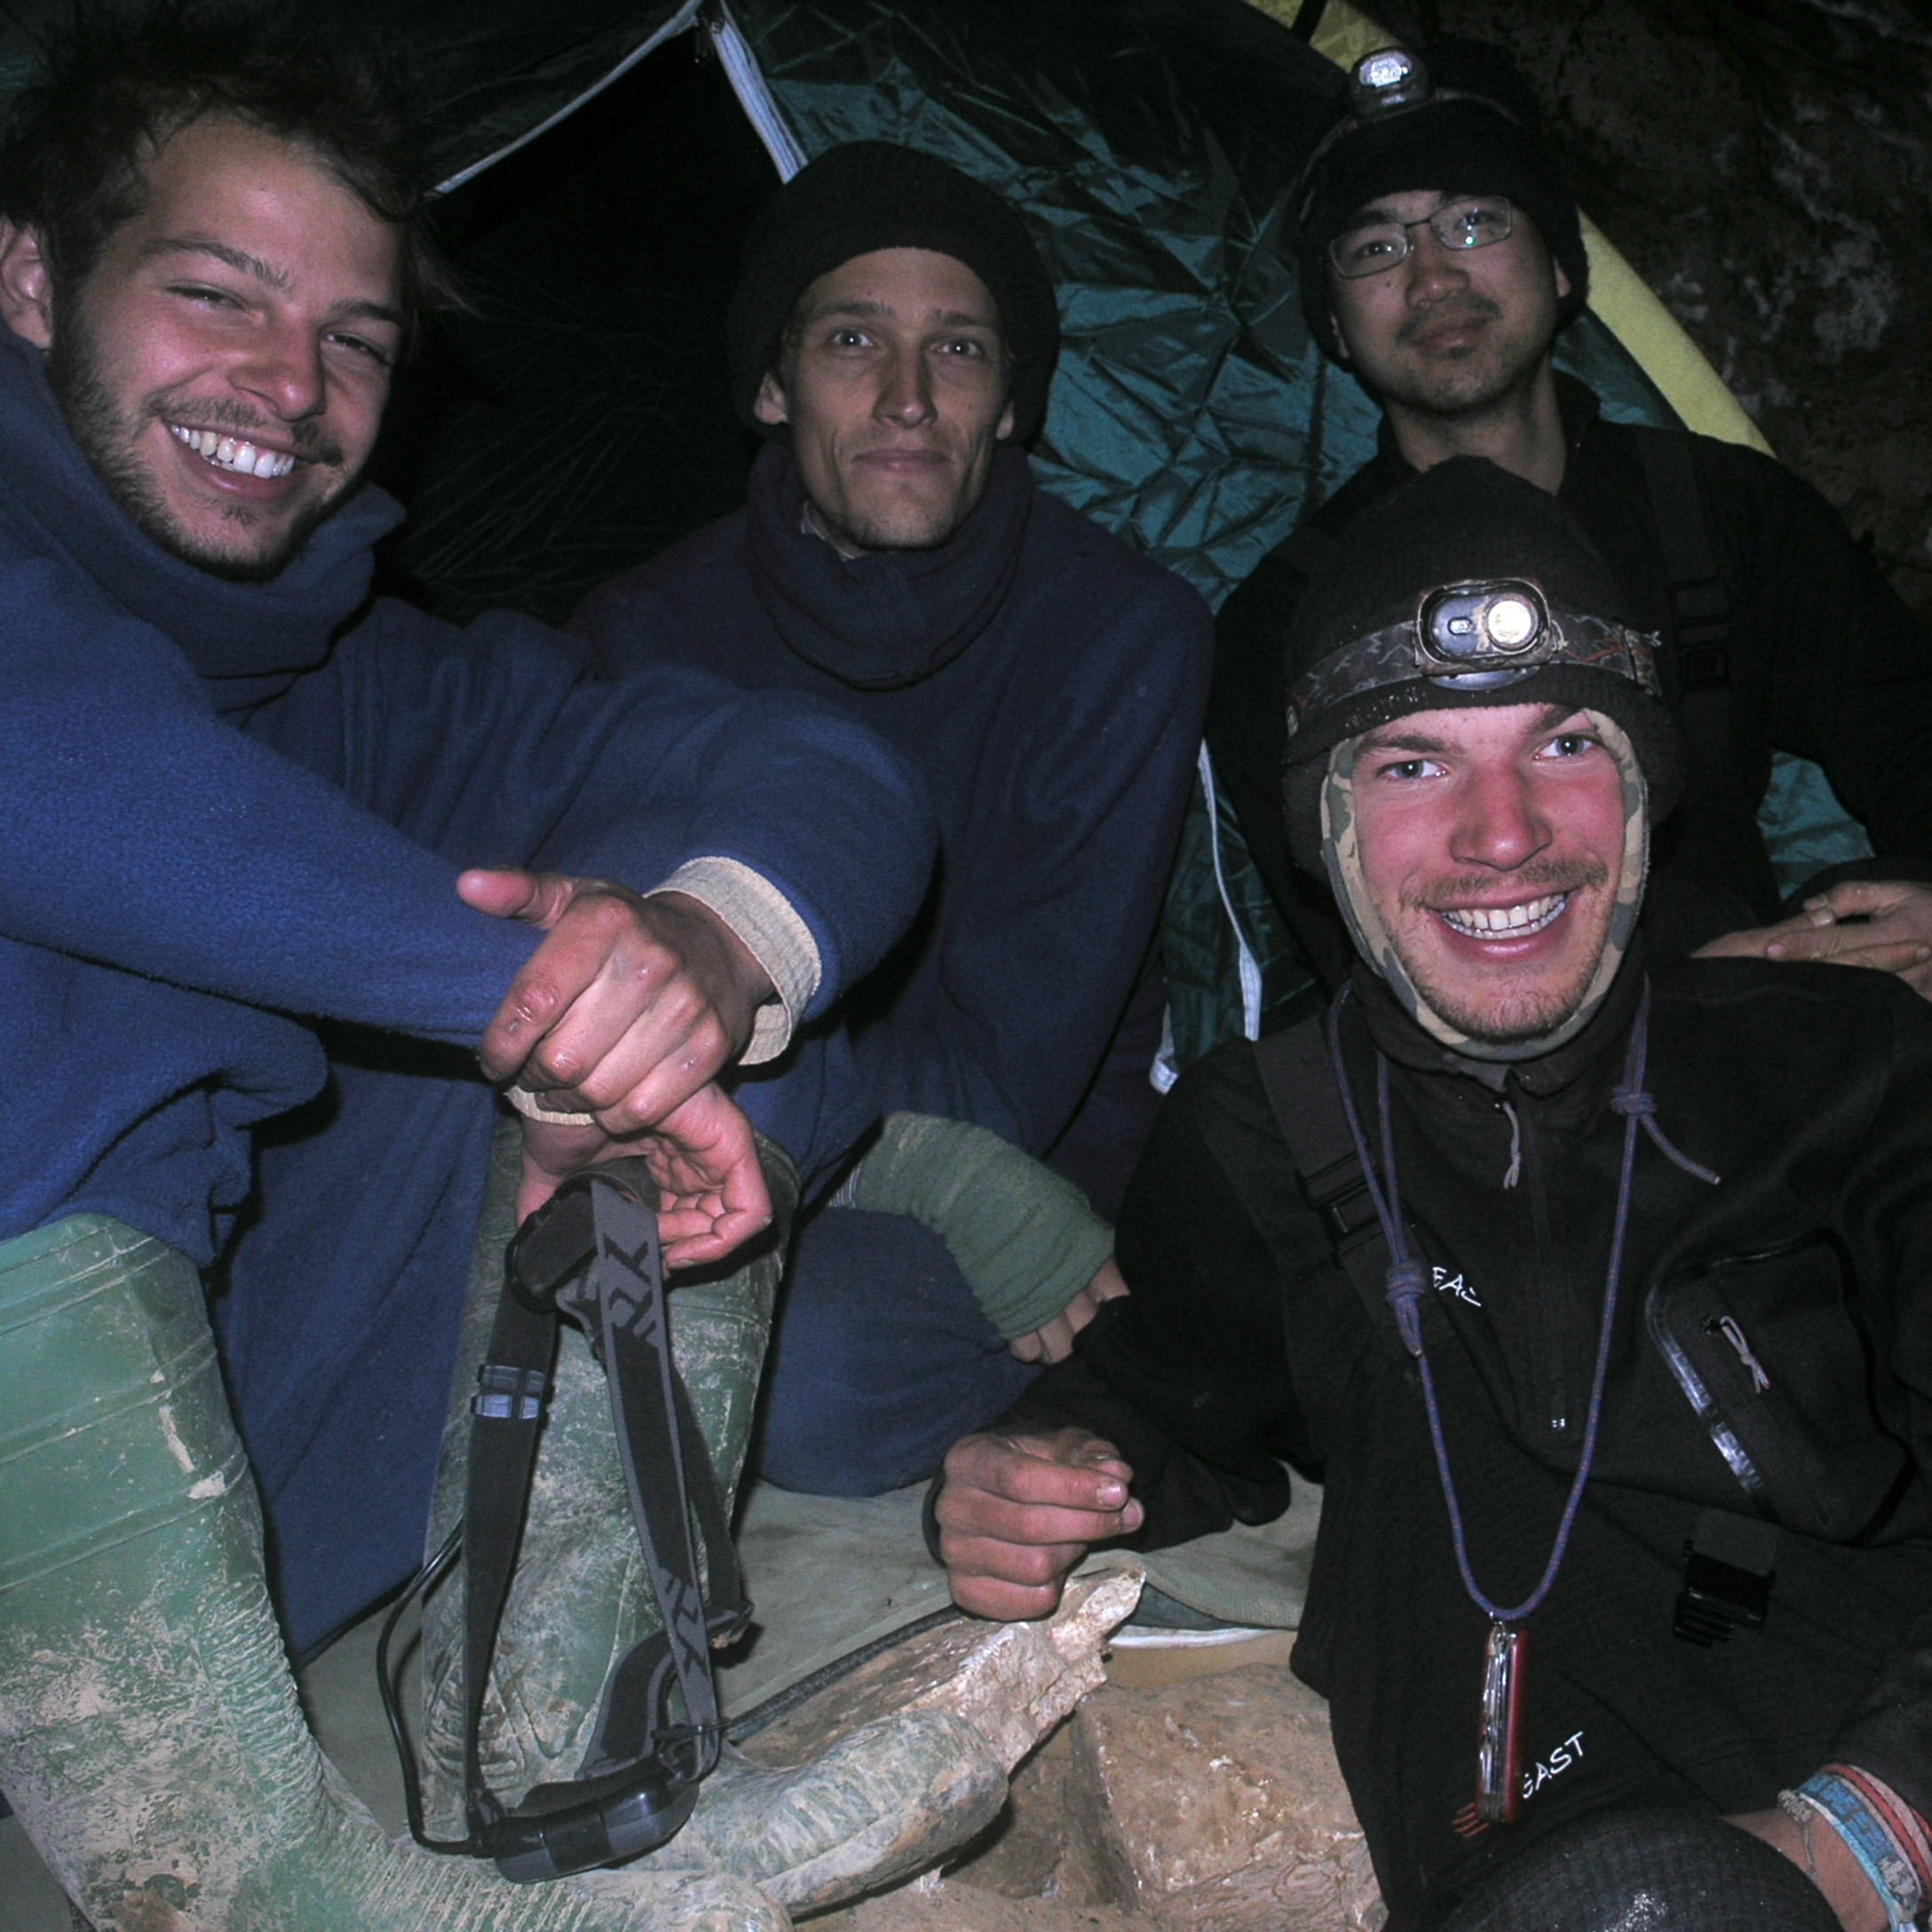
\includegraphics[width=\linewidth]{2010/insomnia/20100806-11-42-40 - Nikolas Kral - P8061854 - Camp X-Ray--orig.jpg}}
        \caption{} \label{myles x-ray}
    \end{subfigure}
    \hfill
     \begin{subfigure}[t]{0.59\textwidth}
        \centering
        \frame{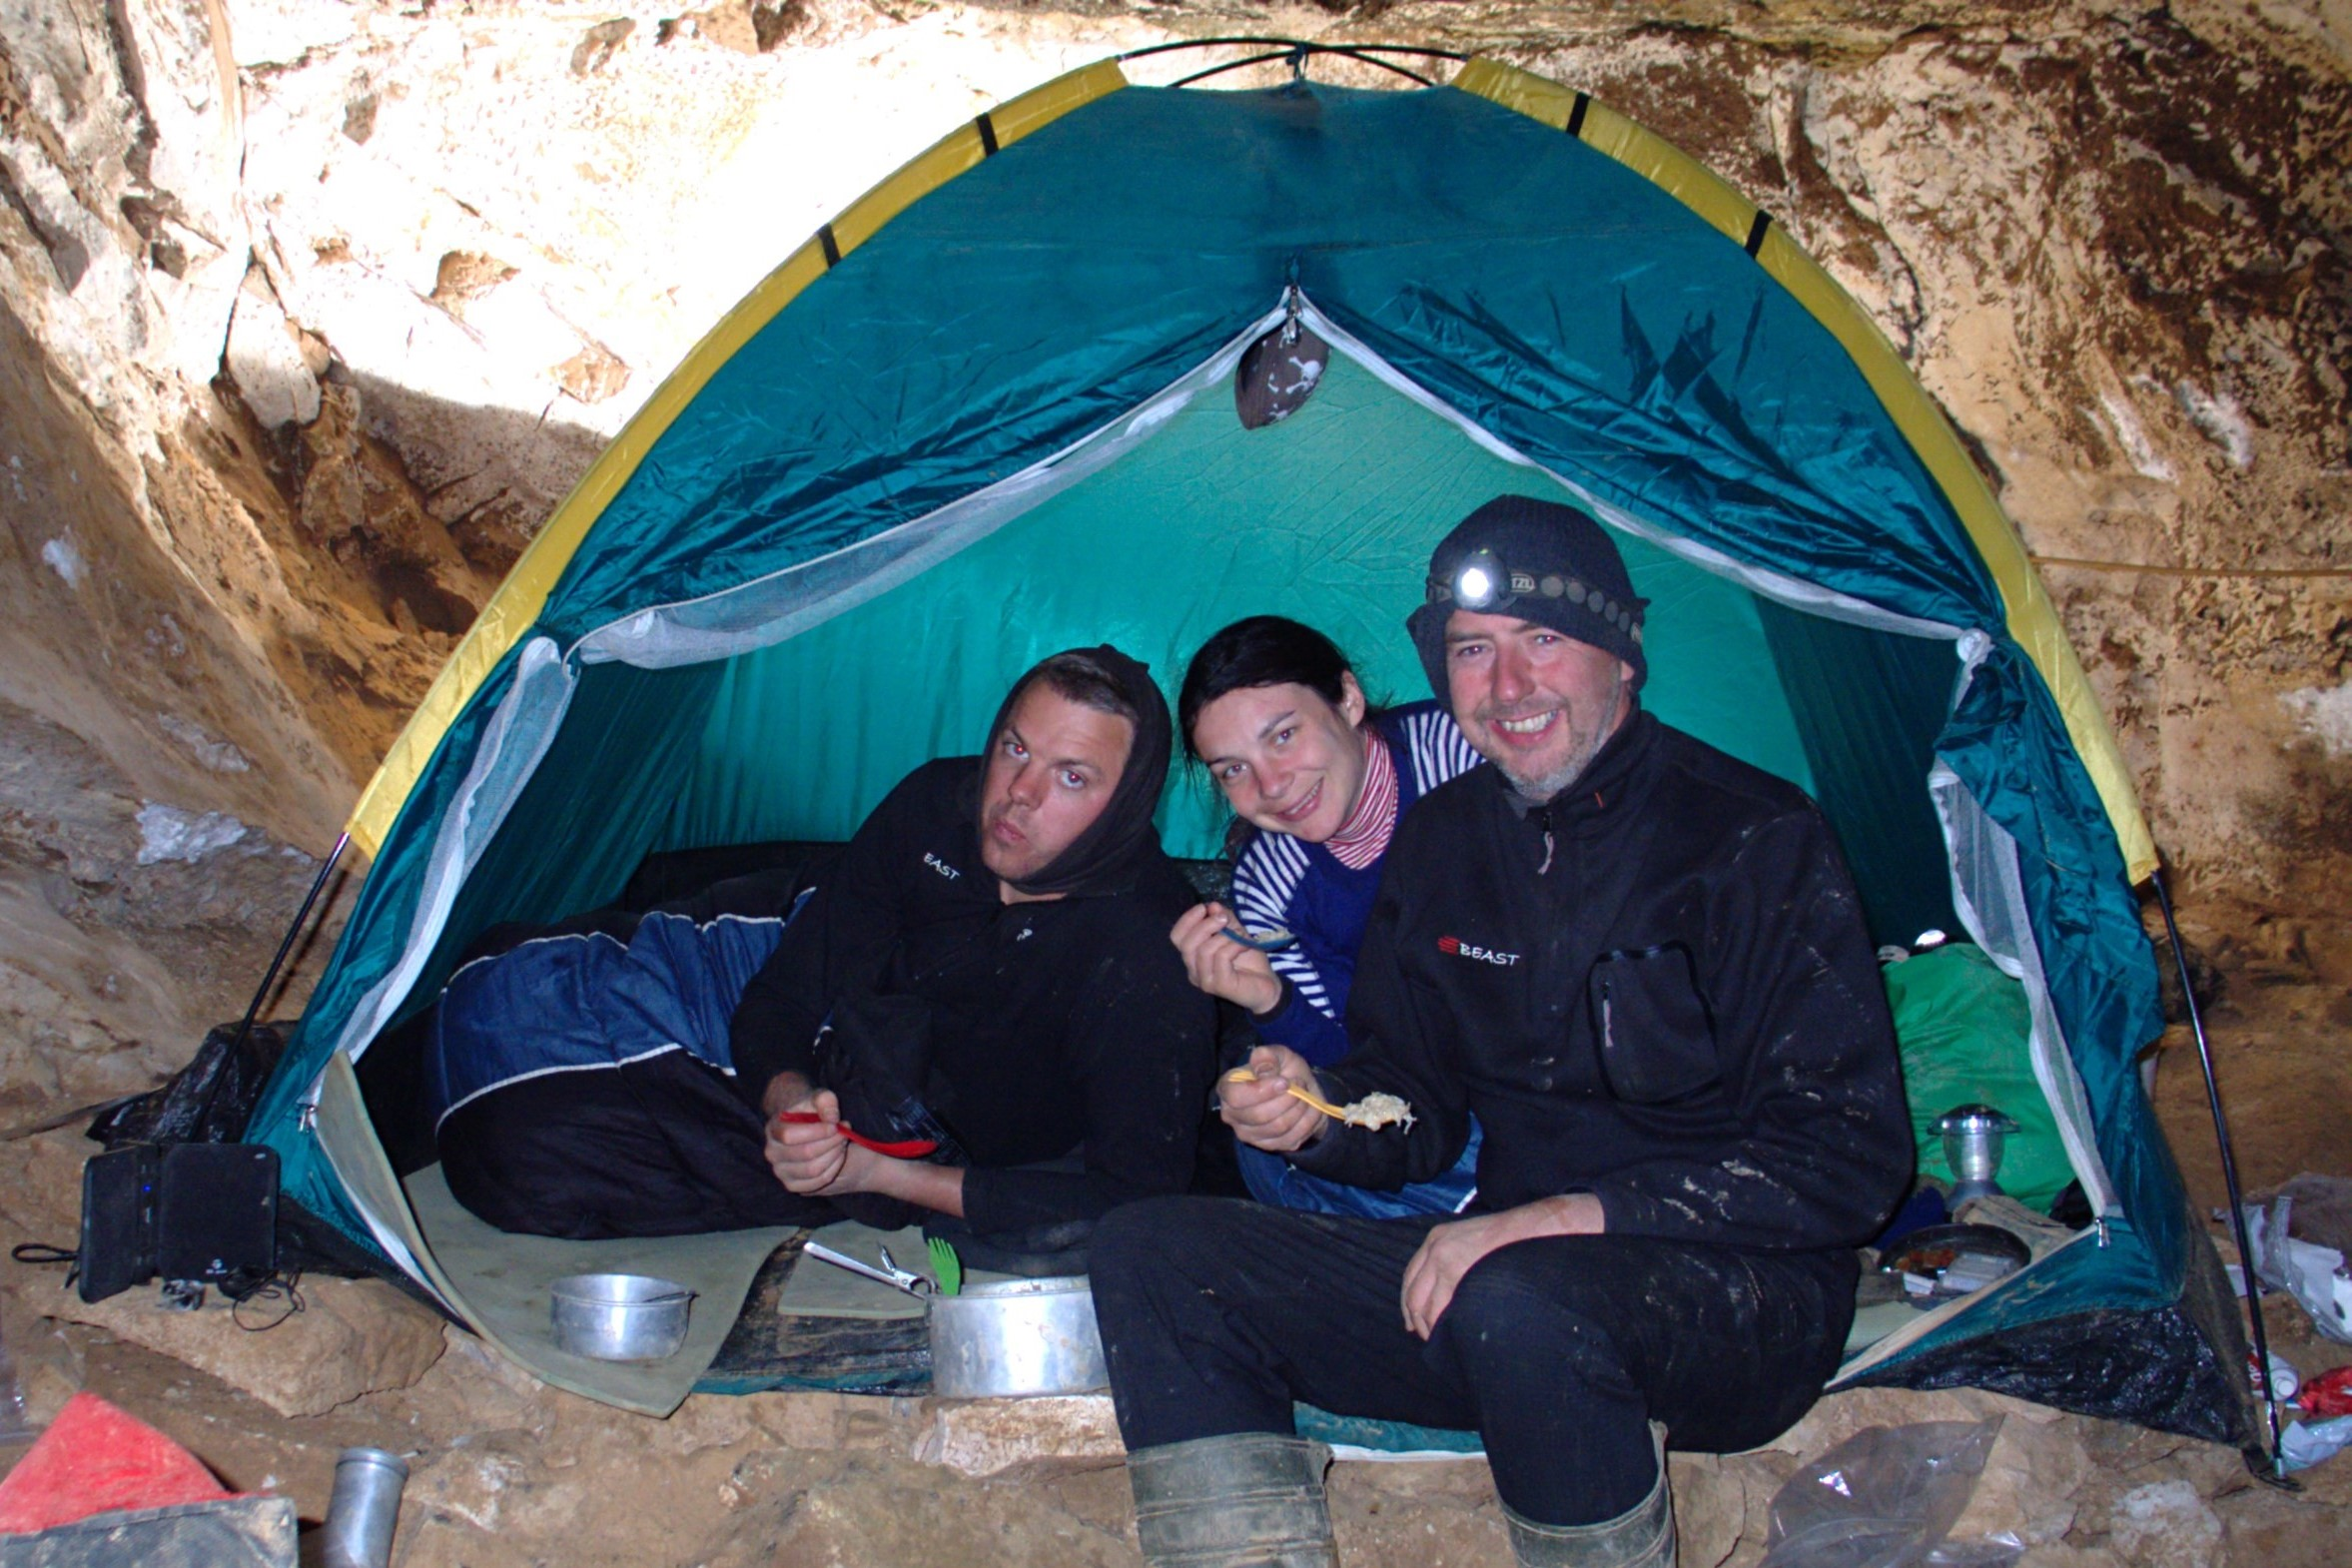
\includegraphics[width=\linewidth]{2010/insomnia/20100731-23-54-22-Jarvist Frost-Canon G5-CRW_0405-Camp X-ray--orig.jpg}}
        \caption{} \label{shed x-ray}
    \end{subfigure}
    
    \vspace{0cm}
    \centering
    \begin{subfigure}[t]{0.59\textwidth}
        \centering
        \frame{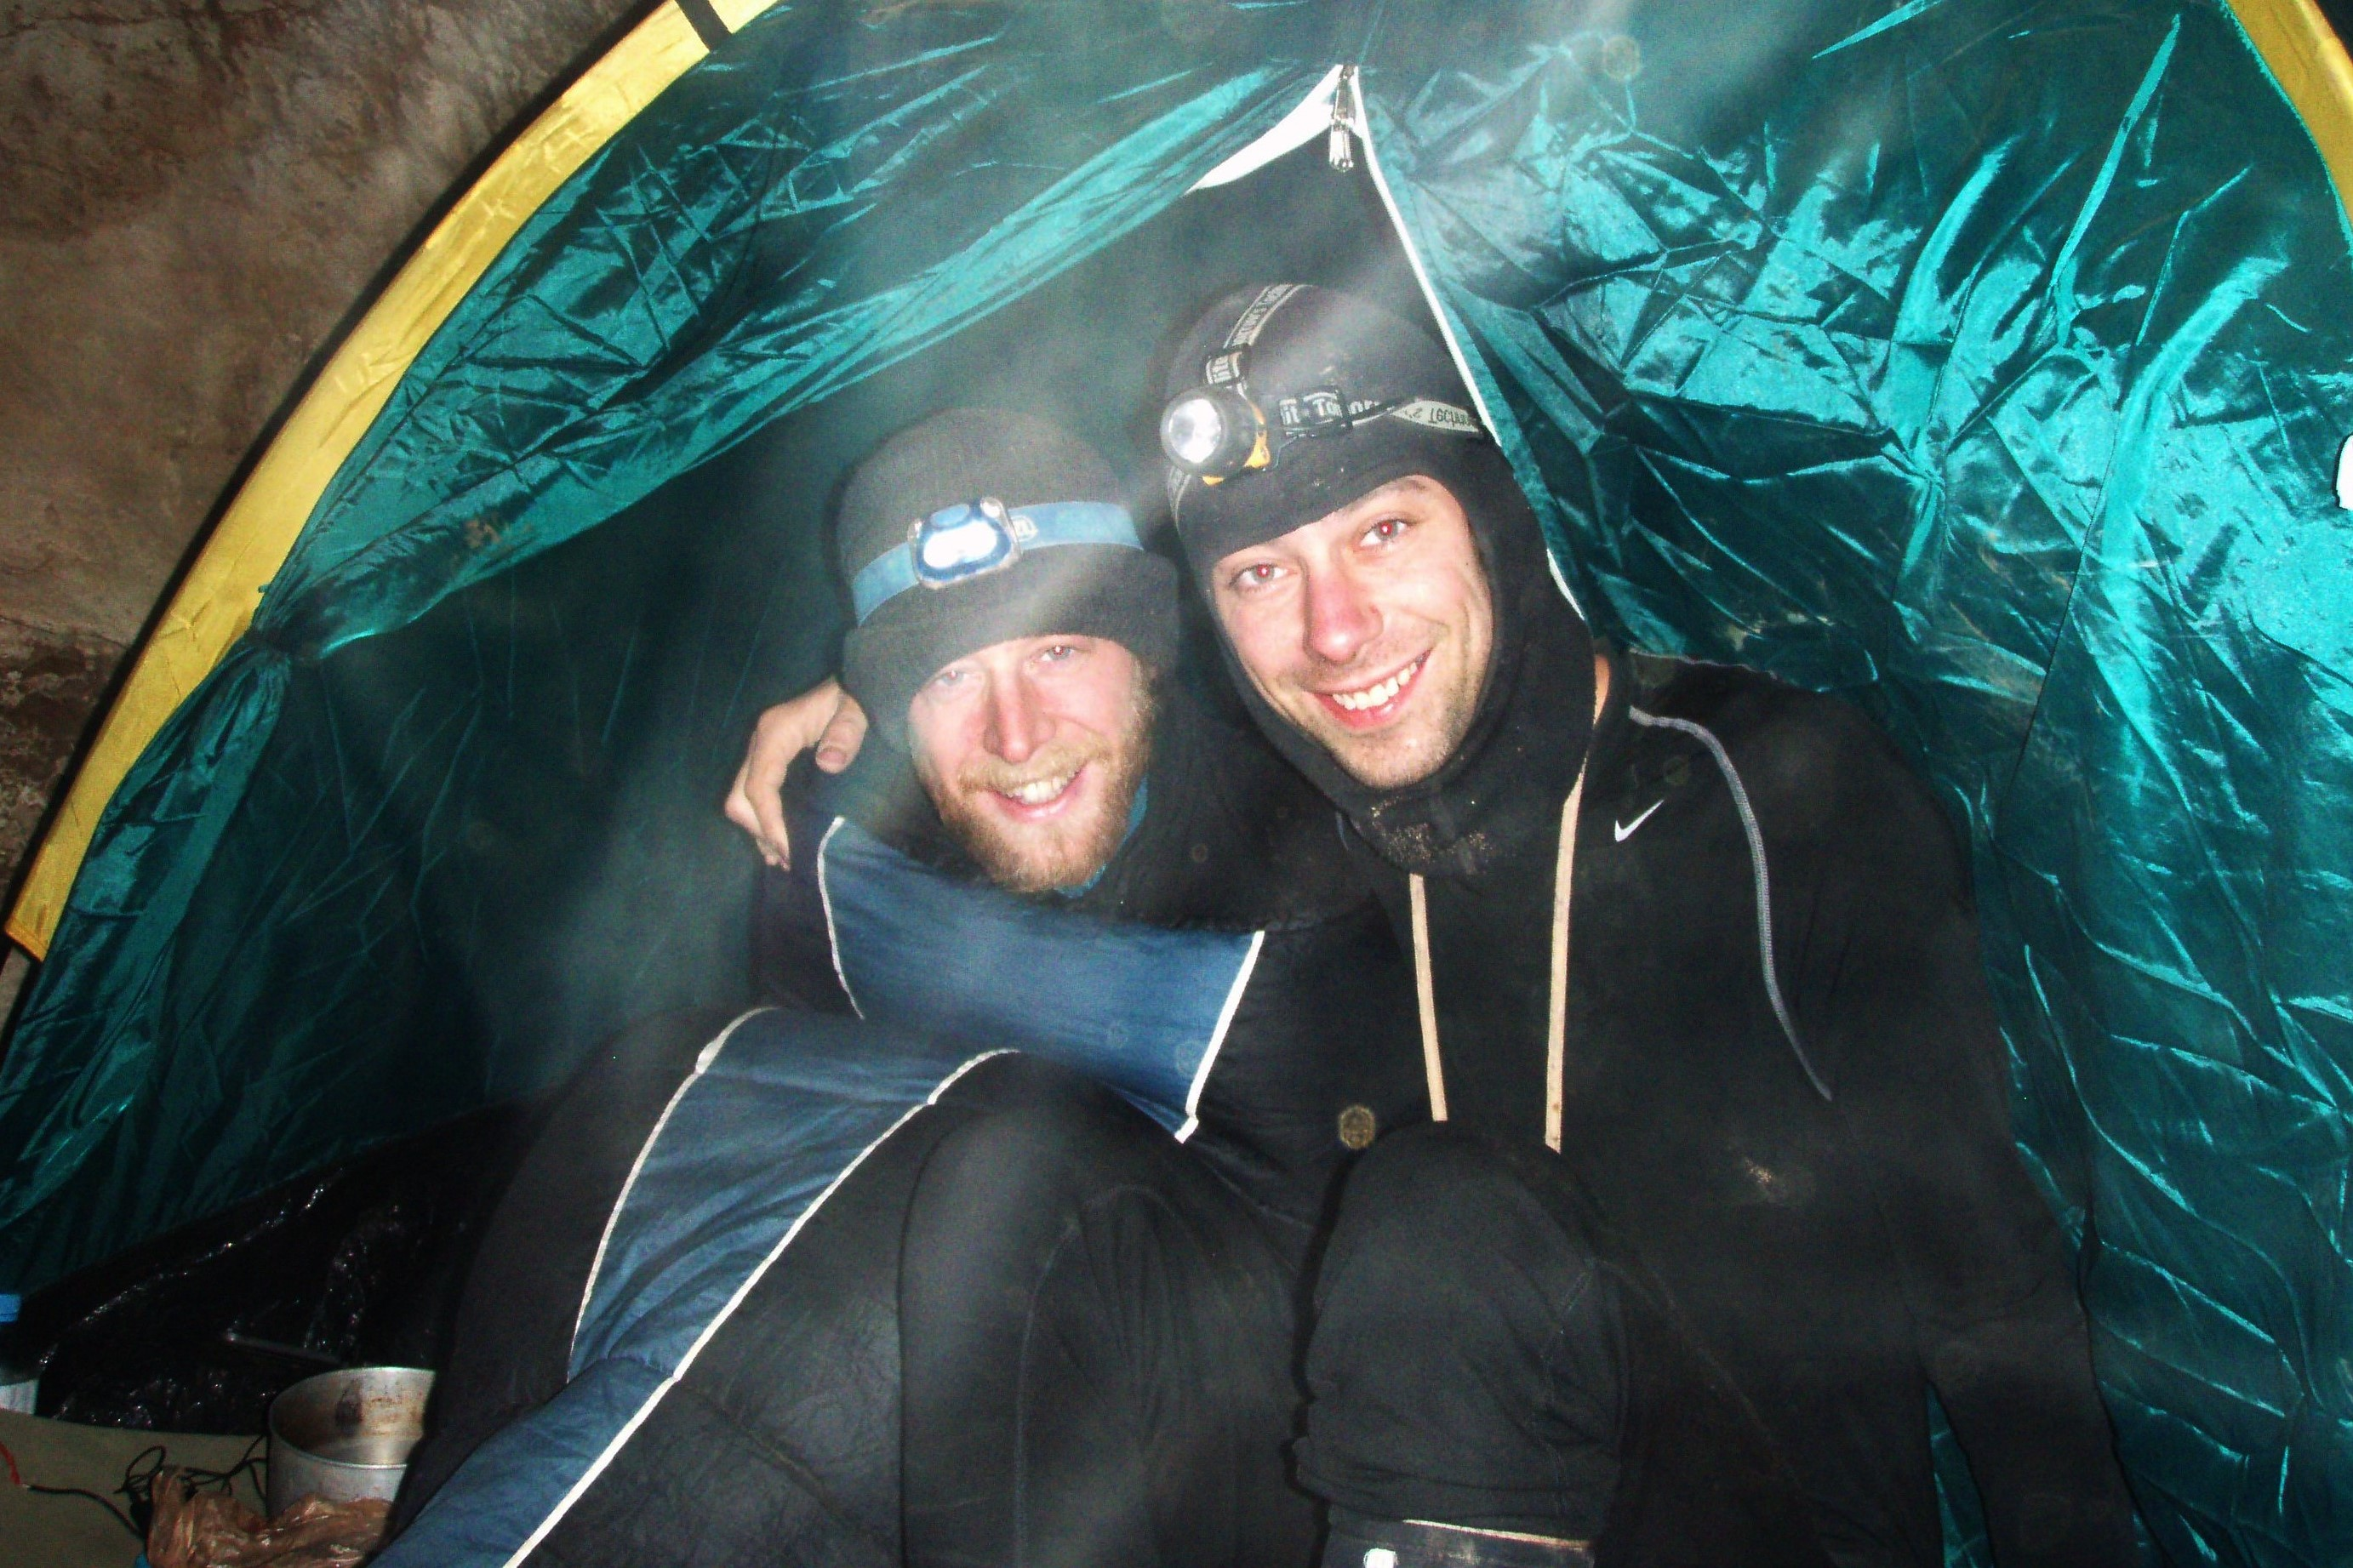
\includegraphics[width=\linewidth]{2010/insomnia/20100807-20-31-33 - Jan Evetts - P2070114 - Camp X-ray--orig.jpg}}
        \caption{} \label{jan x-ray}
    \end{subfigure}
    \hfill
    \begin{subfigure}[t]{0.393\textwidth}
        \centering
        \frame{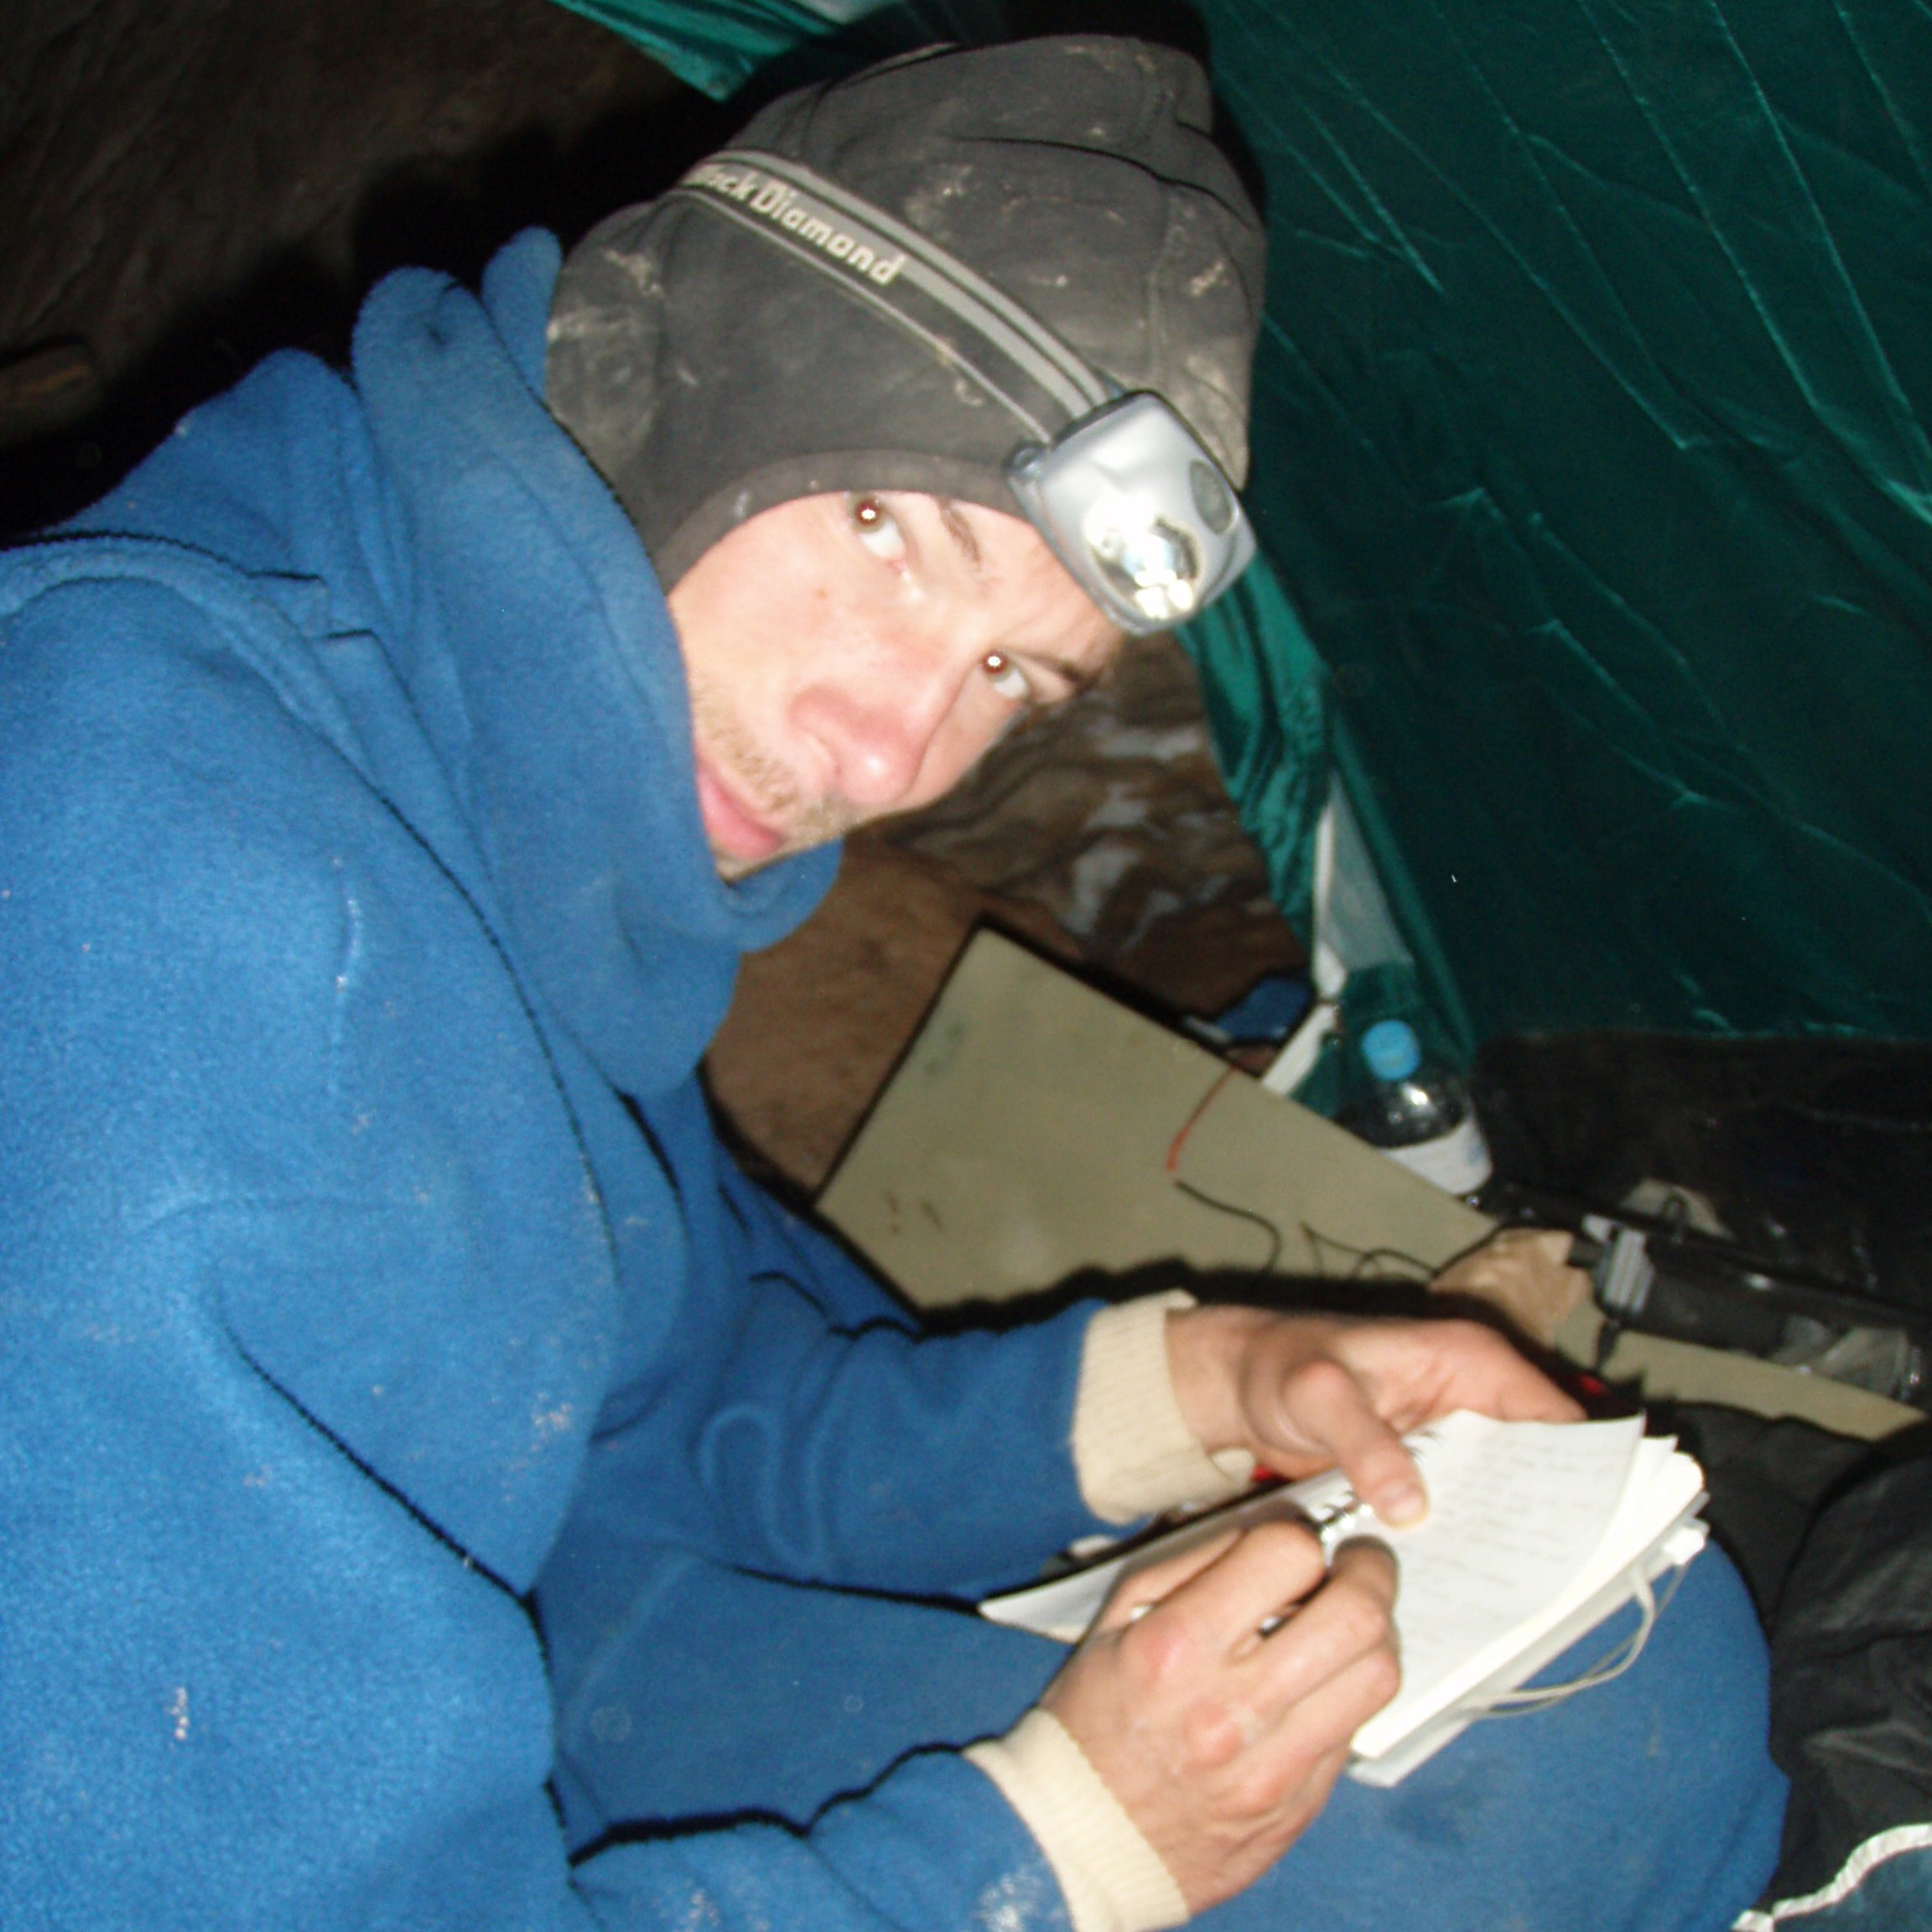
\includegraphics[width=\linewidth]{2010/insomnia/20100807-20-13-04 - Jan Evetts - P2070110 - Camp X-ray--orig.jpg}}
        \caption{} \label{gergely x-ray}
    \end{subfigure}
  
    \vspace{0cm}
    \centering
\begin{subfigure}[t]{0.393\textwidth}
        \centering
        \frame{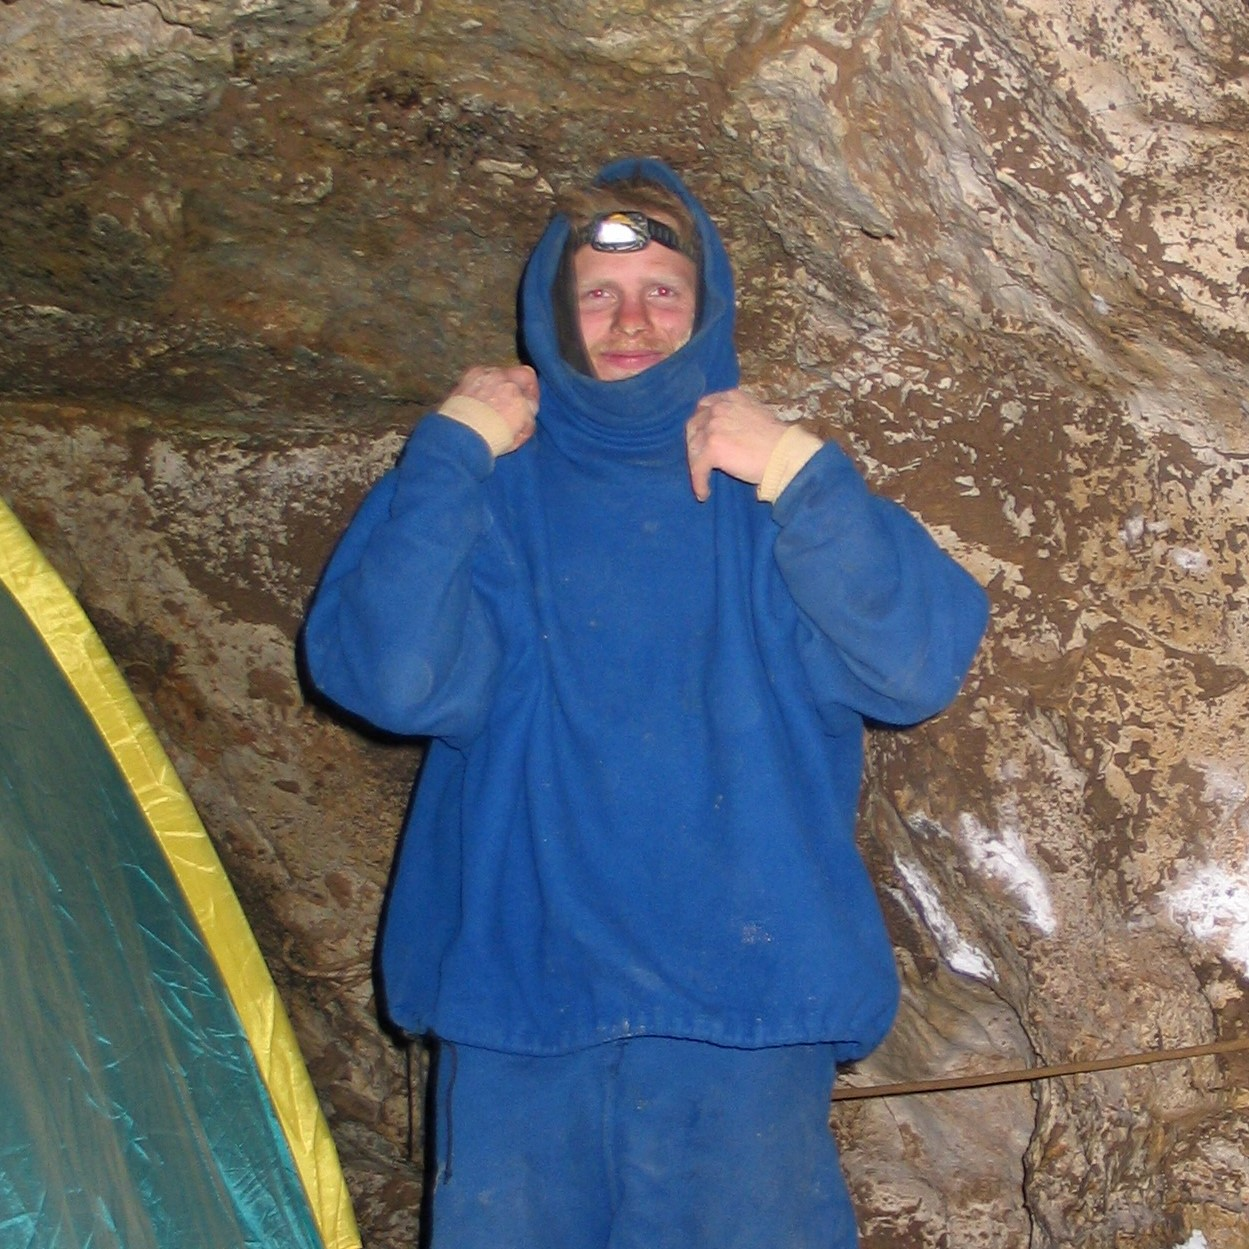
\includegraphics[width=\linewidth]{2010/insomnia/20100806-21-30-51-Jarvist Frost-Canon G5-IMG_0488-Camp X-ray--orig.jpg}}
        \caption{} \label{william x-ray}
    \end{subfigure}
    \hfill
     \begin{subfigure}[t]{0.59\textwidth}
        \centering
        \frame{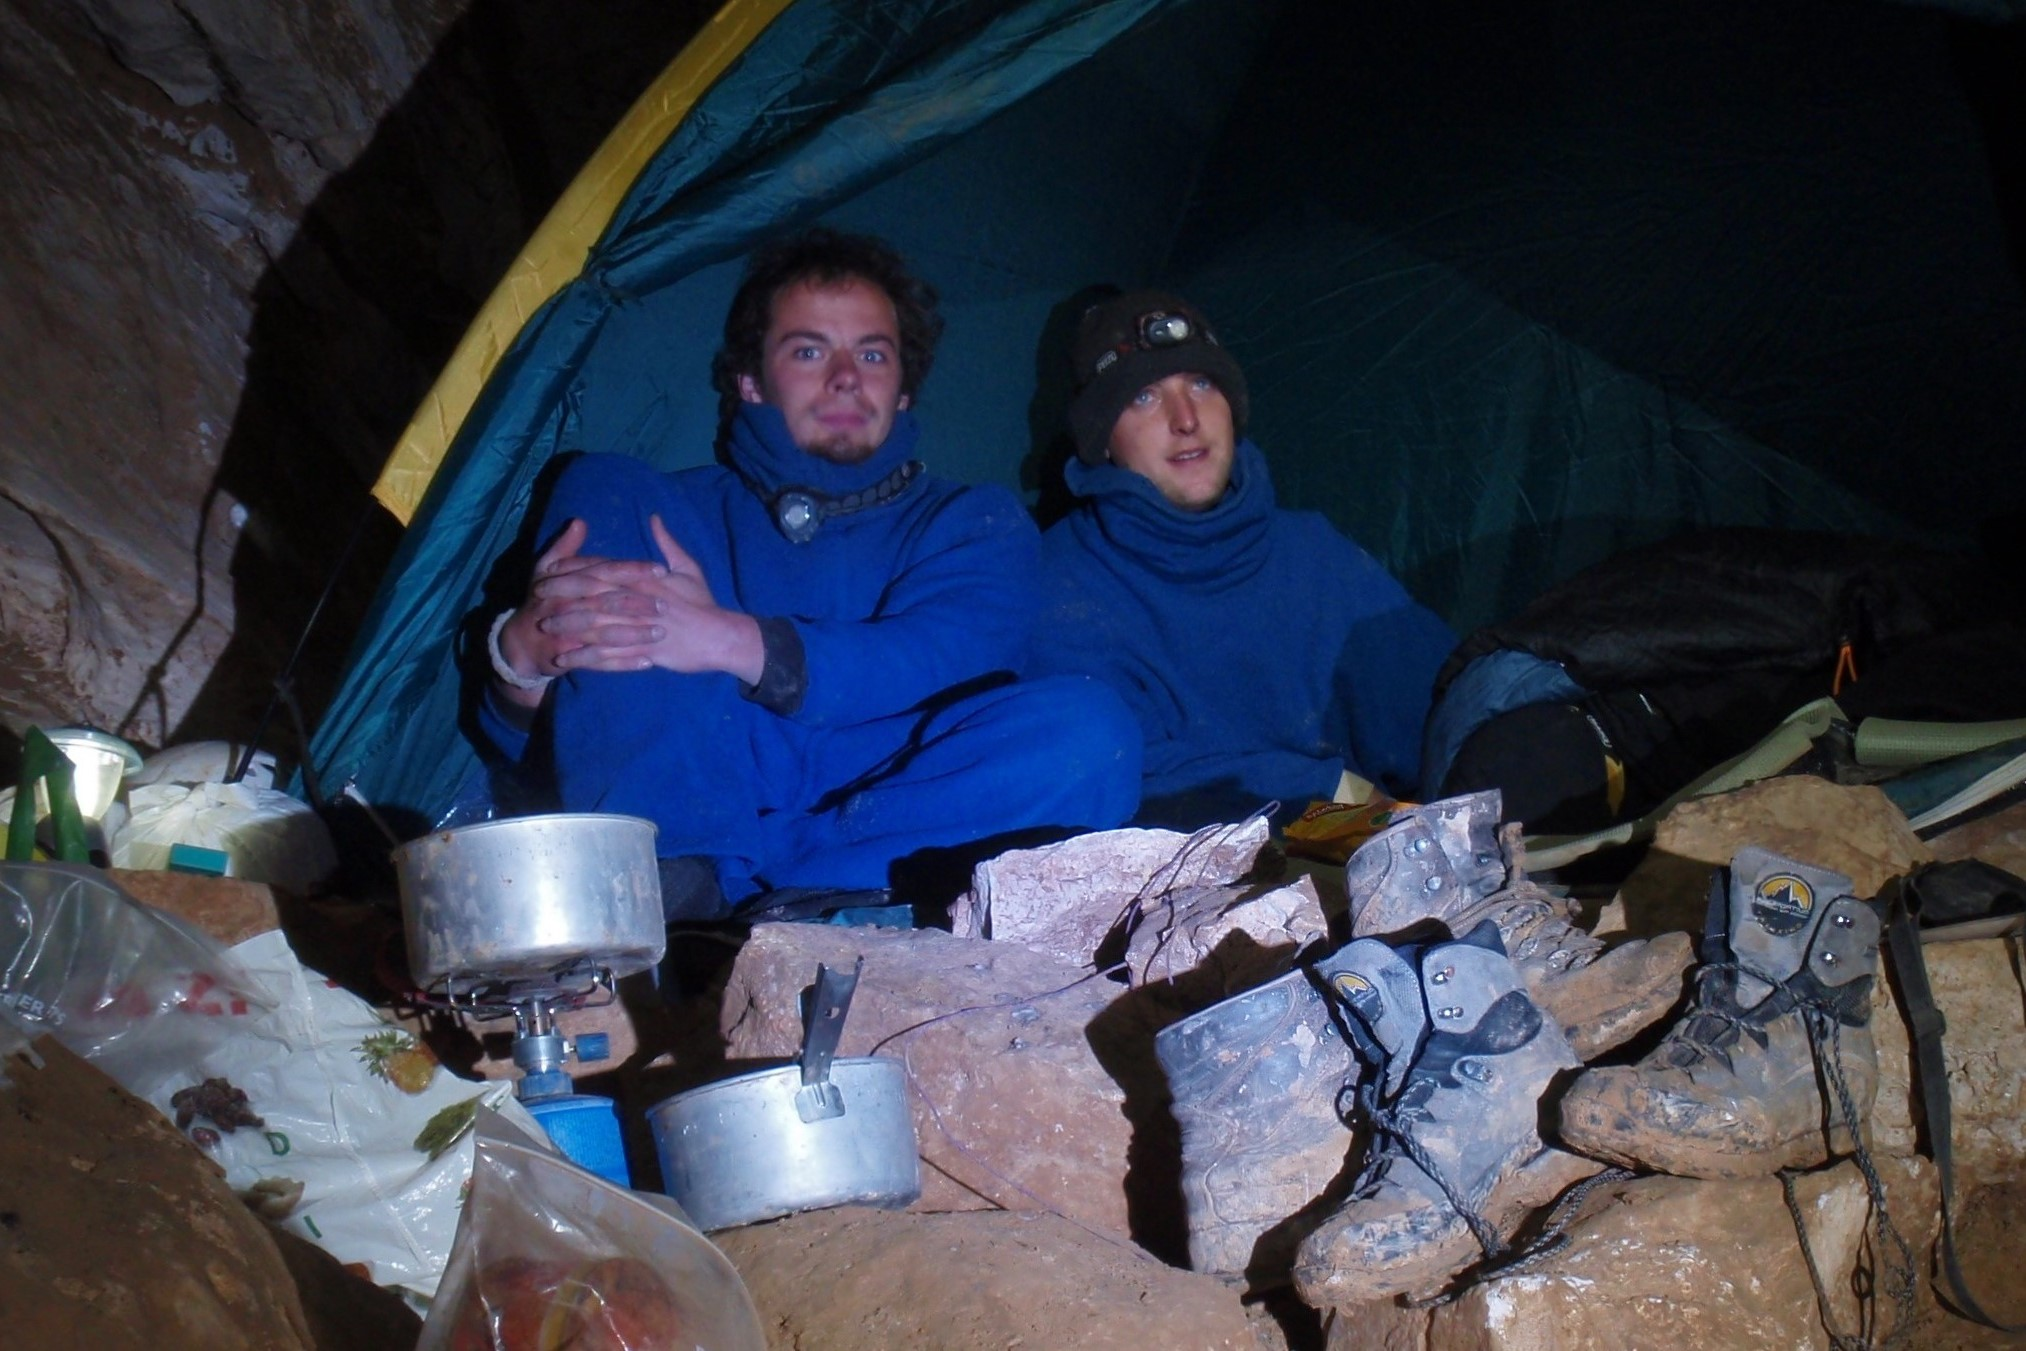
\includegraphics[width=\linewidth]{2010/insomnia/20100802-12-36-45 - Iztok Mozir - P8024768 - Camp X-ray2--orig.jpg}}
        \caption{} \label{maver erik x-ray}
    \end{subfigure}

    \caption{Some of cavers who slept at camp \protect\passage{X-Ray} in 2010.
    \textit{(a)} Myles, Jarv, Thara and Niko. \pic{Nikolas Kral}
    \textit{(b)} Shed, Jana and Martin. \pic{Jarvist Frost}
    \textit{(c)} Jan and James KP. \pic{Jan Evetts}
    \textit{(d)} Gergely making notes. \pic{Izi Možir}
    \textit{(e)} William inside the comf. \pic{Jarvist Frost}
    \textit{(f)} Maver and Erik. \pic{Izi Možir}}
\end{pagefigure}
